\documentclass[11pt,letterpaper]{article}

\usepackage[spanish,es-tabla,es-nodecimaldot]{babel}
\usepackage{amsmath}
\usepackage[utf8]{inputenc}
\usepackage[T1]{fontenc}
\usepackage{lmodern}
\usepackage{graphicx}
\usepackage{listings}
\usepackage{anysize} 
\usepackage{fancyhdr}
\usepackage{amsmath}
\usepackage{pdfpages}
\usepackage{graphics}
\usepackage{capt-of}
\usepackage{tabularx}
\usepackage{rotating}
\usepackage{tikz}
\usepackage[colorlinks=true,plainpages=true,citecolor=blue,linkcolor=blue]{hyperref}


\marginsize{2cm}{2cm}{2cm}{2cm}
\pagestyle{fancy}
\fancyhf{Sistemas celulares}
\fancyhead[L]{\footnotesize UPIITA-IPN} 
\fancyhead[R]{\footnotesize 2TV7} 
\fancyfoot[R]{\footnotesize Tarea 3}
\fancyfoot[C]{\thepage}
\fancyfoot[L]{\footnotesize } 

\renewcommand{\footrulewidth}{0.4pt}
\renewcommand{\spanishtablename}{Tabla}
\renewcommand{\labelitemii}{$\star$}
\graphicspath{ {C:/Users/Anselmo/Documents/GitHub/upiita-SistemasCelulares/Tarea3/imagenes} }

\begin{document}


\includepdf[pages={1}]{Portada}

\newpage
\tableofcontents
\listoffigures
\listoftables

\newpage
\section{Desarrollo}
La población actual del municipio de Nezahualcóyotl es de 1,228,54 habitantes.
La población con la cual se realizó el estudio anterior corresponde al 5\% de 
la población actual. El resultante de esta operación es de 61,432 habitantes. 
\\ \\
Para el siguiente estudio se propone que el aumento de población de los 80s 
sea de un 1.5\%. Este supuesto se hace pensando en el cambio de D-AMPS a GSM y 
a que este aumento de población se le proporcionará servicio. El 1.5\% de la 
población de los 80s es 92,149. El total de población para el estudio actual 
es de 153,581 habitantes.
\\ \\
Uno de los puntos a resaltar en el cambio de AMPS a GSM es el cambio del 
método de acceso de división de frecuencia por división de tiempo. Ahora todas 
las células del clúster trabajaran sobre la misma banda de frecuencias. Para 
obtener el numero de canales con este nuevo método, se parte de tres datos 
que fueron obtenidos en AMPS del estudio anterior, los canales de AMPS, los 
Erlang y el número de llamadas a proporcionar.
\\ \\
Los datos del estudio anterior se enlistan a continuación.
\begin{itemize}
    \item CH: 2010.
    \item N: 49,618.2.
    \item A: 2480.91.
\end{itemize}

Para obtener el numero de canales en TDMA se debe de multiplicar los canales 
en AMPS.

\begin{equation}
    nTDMA=CH_{AMPS} \ * \ 8
\end{equation}

\begin{figure}[ht]
    \centering
    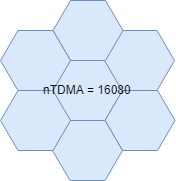
\includegraphics[width=0.4\textwidth]{imagenes/cluster.png}
    \caption{Total de canales en el clúster.}
\end{figure}


\newpage
Posteriormente se puede calcular lambda con la siguiente expresión, que es la 
intensidad de tráfico. Se propone que hp sea 3600 segundos.

\begin{equation}
    \lambda=\frac{N}{hp}=\frac{49618.2}{3600}=13.782
\end{equation}
\\ \\
Retamando el tiempo promedio $\overline{t}$, se obtiene la tasa de espera $\mu$ 
con la siguiente expresión. 

\begin{equation}
    \mu=\frac{1}{\overline{t}}=\frac{1}{180} \ ms
\end{equation}
\\ \\
Los datos obtenidos anteriormente servirán para calcular los parámetros que entrega 
la distribución de Poisson. En seguida se muestra un diagrama con los parámetros que se 
obtendrán.


\begin{figure}[ht]
    \centering
    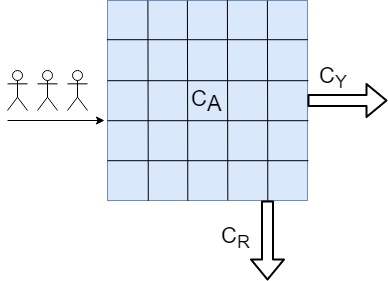
\includegraphics[width=0.7\textwidth]{imagenes/pos.png}
    \caption{Parámetros que entrega la distribución de Poisson.}
\end{figure}

\newpage
Primero se calcula las gestionadas atendidas $C_{A}$ con la siguiente expresión.
\begin{equation}
    C_A=n_{TDMA} \ * \ \lambda = 49618.2 * 13.782= 683,838.0324
\end{equation}

Ahora las llamadas cursadas $C_Y$.
\begin{equation}
    C_Y=C_A(1-B)=683,838.0324(1-0.01)=676,999.6521
\end{equation}

Por ultimo las llamadas rechazadas.
\begin{equation}
    C_R=C_A*B=683,838.0324*0.01=6,838.38
\end{equation}

Con la información anterior se puede obtener las gestiones efectivas.
\begin{equation}
    C_A-C_R=683,838.0324-6,838.38=676,699.6524
\end{equation}

En la siguiente tabla se concentran los resultados obtenidos.
\begin{table}[ht]
    \centering
    \begin{tabular}{|c|c|}
    \hline
    Parámetro & Valor   \\ \hline
    $C_A$ & $683,838.0324$  \\ \hline
    $C_Y$ & $676,999.6521$  \\ \hline
    $C_R$ & $6,838.38$  \\ \hline
    Gestiones efectivas & $676,699.6524$  \\ \hline
    \end{tabular}
    \caption{Tabla de resultados.}
    \label{tab:my-table}
\end{table}

\section{Conclusiones}

\end{document}